
\documentclass[final,hyperref={pdfpagelabels=false}]{beamer}
\mode<presentation>{\usetheme{VUW}}
\usepackage{times}
\usepackage{amsmath,amsthm, amssymb, latexsym}
\usepackage[english]{babel}
\usepackage[latin1]{inputenc}
\usepackage[orientation=portrait,size=a0,scale=1.3,debug]{beamerposter}
\usepackage{natbib}
\usepackage{enumitem}
\usepackage{adjustbox}
\usepackage{ragged2e} 

%%%%%%%%%%%%%%%%%%%%%%%%%%%%%%%%%%%%%%%%%%%%%%%%%%%%%%%%%%%%%%%%%%%%%%%%%%%%%%%%%5
\graphicspath{{figures/}}
\title{The Puoko-nui CCD Time Series Photometer}
\author[Chote \& Sullivan]{P. Chote \& D. J. Sullivan}
\institute{School of Chemical and Physical Sciences, Victoria University of Wellington}

%%%%%%%%%%%%%%%%%%%%%%%%%%%%%%%%%%%%%%%%%%%%%%%%%%%%%%%%%%%%%%%%%%%%%%%%%%%%%%%%%5

\begin{document}
	\centering
	\begin{frame}{} 
		\vskip -1.5ex
		% A fudge to center the column titles relative to the edge of the page
		\begin{adjustbox}{minipage=0.99\linewidth, margin=22pt 0pt 0pt 0pt,center}
			\begin{columns}[t]
				\begin{column}{.66\linewidth}
					\begin{block}{\large Instrument Overview}
						\justifying
						%!TEX root = /Users/paul/phd/talks/WD12poster/puokonui-poster.tex
\vspace{-1.75cm}
\begin{itemize}[itemsep=20pt]
% high speed precision time series photometer?
\item[] Puoko-nui is a precision time series photometer developed at Victoria
University of Wellington, primarily for use with the 1m McLellan
telescope at Mt John University Observatory (MJUO), Lake Tekapo, New Zealand.
It has been operating in its current form since early 2011.

\item[] The initial design concept for the photometer was inspired by an
earlier instrument (Argos) developed at the University of Texas in Austin.
Puoko-nui features a modular design which replaces the parallel port timer
dongle in Argos with a separate programmable hardware unit to provide a clean
separation of timing and acquisition, and allow for much greater flexibility
in operation.

\end{itemize}
\vspace{-1.75cm}
					\end{block}
					\begin{block}{\large Detectors}
						\justifying
						%!TEX root = /Users/paul/phd/talks/WD12poster/puokonui-poster.tex
\vspace{-1.75cm}
\begin{itemize}[itemsep=20pt]
	
\item[] Puoko-nui has two CCD detectors. The primary detector is a shutterless
1k\,$\times$\,1k pixel frame-transfer CCD that is part of a Princeton Instruments
Micromax camera system.  A smaller SBIG ST-402ME CCD is mounted in an
offset guiding position with a 2D slide mechanism, which allows a bright star
outside the main field of view to be imaged independently of the main detector
for telescope autoguiding. Both detectors connect to their respective control PCs
via USB.

\item[] The frame-transfer operation of the primary CCD effectively eliminates
readout deadtime, allowing the system to be run without a shutter. At the
maximum 1\,MHz readout rate, full-resolution exposures as short as 2 seconds
are possible. Faster rates can be achieved by binning pixels. The CCD is
thermoelectrically cooled to $-50^\circ$C to reduce thermal noise.

\item[] Our white dwarf observations use a broad blue band
BG40 filter to reduce the sensitivity to red sky photons.
The primary CCD is normally operated with 2\,$\times$\,2 pixel binning and 100\,kHz 
readout to minimize noise. 

\item[] Paired with the MJUO 1m telescope at f/8, the primary field of view is
5.7 square arcminutes. When operated with 2\,$\times$\,2 binning, the aggregate
pixels each image a 0.66 square arcsecond region of the sky.

\end{itemize}
\vspace{-1.75cm}
					\end{block}
				\end{column}
				\begin{column}{.3\linewidth}
					\vskip 0.2ex
					\begin{beamercolorbox}[rounded=false,shadow=false,colsep*=.75ex,sep=.75ex,vmode]{block body}%
	    				\ifbeamercolorempty[bg]{block body}{\vskip-.25ex}{\vskip-.75ex}\vbox{}%
						\centering
						\includegraphics[width=0.95\textwidth]{figures/instrument}\\
						\small Puoko-nui attached to the 1m McLellan Telescope at\\ Mt John University Observatory, Lake Tekapo, NZ
	  				\end{beamercolorbox}
				\end{column}
			\end{columns}
			\vskip 1ex
			\begin{columns}[b]
				\begin{column}{.50\linewidth}
					\begin{beamercolorbox}[rounded=false,shadow=false,colsep*=.75ex,sep=.75ex,vmode]{block body}%
	    				\ifbeamercolorempty[bg]{block body}{\vskip-.25ex}{\vskip-.75ex}\vbox{}%
						\centering
						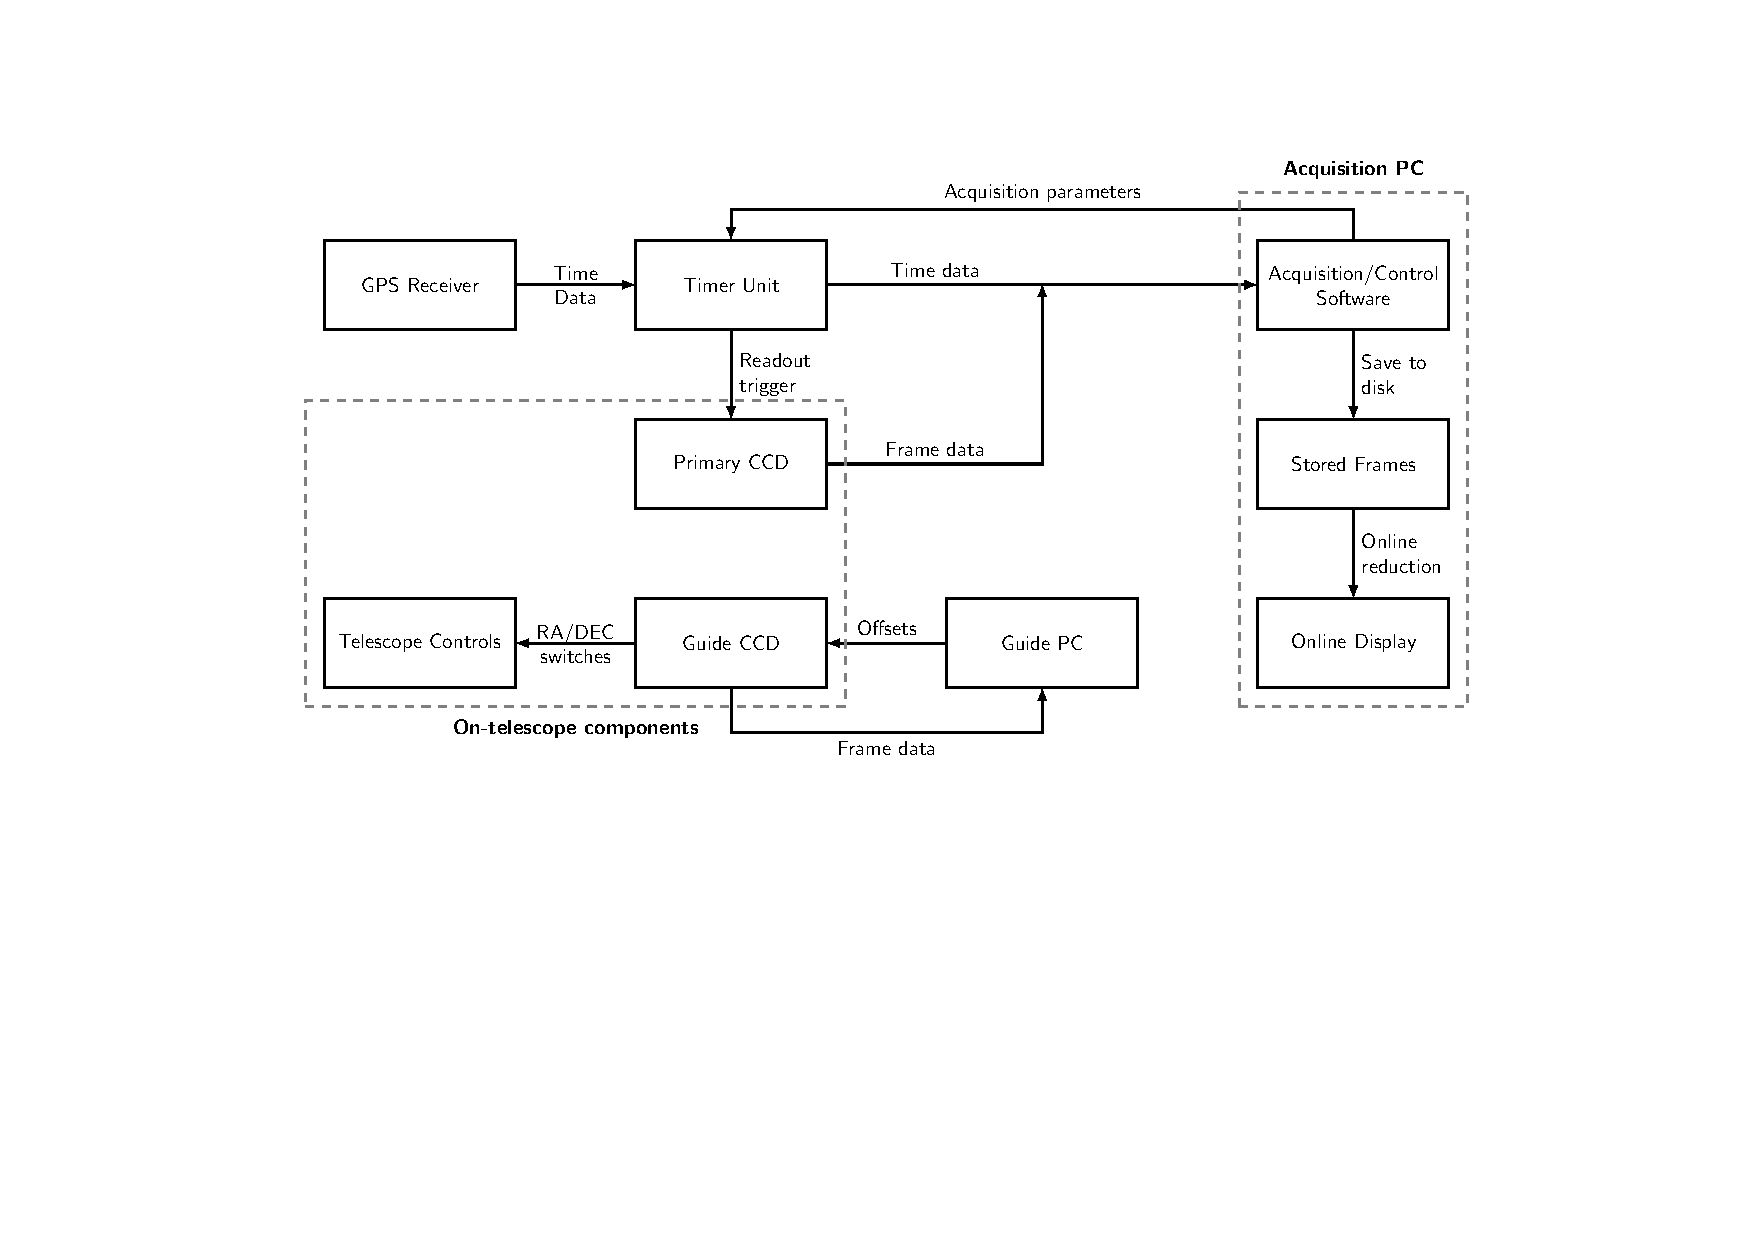
\includegraphics[width=0.9\textwidth, trim=5.3cm 8cm 5cm 2cm]{figures/equipment-block}\\
						\small Block diagram illustrating the main components of the instrument
					\end{beamercolorbox}
					\vskip 2ex
					\begin{block}{\large Acquisition}
						\justifying
						%!TEX root = /Users/paul/phd/talks/WD12poster/puokonui-poster.tex
\vspace{-1.75cm}
\begin{itemize}[itemsep=20pt]
\item[] The instrument control and online reduction software is run on a pair of
compact ``net-top'' PCs situated adjacent to the telescope and controlled via a remote
connection. One PC runs the acquisition and online reduction software
in an Ubuntu GNU/Linux environment. The other runs the proprietary SBIG
acquisition/autoguiding software in a Microsoft Windows environment.

\item[] The acquisition software provides facilities for setting image metadata
(target name, observers, etc) and configuring run parameters such as exposure
time and CCD temperature.

\item[] The software acts as a passive receiver once an acquisition run
commences, tagging each frame with the GPS timestamp and image metadata. 
Frames are saved to disk as compressed FITS files.

\end{itemize}
\vspace{-1.75cm}
					\end{block}
					\begin{block}{\large Online Reduction}
						\justifying
						%!TEX root = /Users/paul/phd/talks/WD12poster/puokonui-poster.tex
\vspace{-1.75cm}
\begin{itemize}[itemsep=20pt]
\item[] We have also created a software package for online reduction and analysis
of Puoko-nui data, called \texttt{tsreduce}.

%\item[] We have developed a robust set of online reduction and analysis
%software for Puoko-nui, called \texttt{tsreduce}.

\item[] \texttt{tsreduce} performs aperture photometry on selected target and
comparison stars. The intrinsic variation in the target star (measured in
milli-modulation amplitudes; 10\,mma~=~1\% change) is determined by taking the
ratio of the target and comparison intensities, then subtracting a low-order 
polynomial fit to\\remove any residual long-period effects.

\item[] Frames are processed immediately after acquisition, producing an up to date
graphical display of the raw lightcurves for each star, and a lightcurve and Fourier
amplitude spectrum of the intrinsic target intensity.

\item[] Offline analysis functionality includes routines for optimizing aperture size,
BJD timestamp corrections, and Fourier analysis techniques including prewhitening.

%\item[] Source code (GPLv3 licensed) is available online at
%\url{https://github.com/pchote/tsreduce}

\end{itemize}
\vspace{-1.75cm}
					\end{block}
				\end{column}
				\begin{column}{.46\linewidth}
					\begin{block}{\large Timing}
						\justifying
						%!TEX root = /Users/paul/phd/talks/WD12poster/puokonui-poster.tex
\vspace{-1.75cm}
\begin{itemize}[itemsep=20pt]

\item[] Exposure timing is controlled by a custom-built unit based around the
ATmega1284p microcontroller. Timing information is received from an external
GPS receiver via RS232 and a 1\,Hz edge-aligned time pulse.

\item[] Camera readouts are triggered via a BNC cable connection, with a second
connection used for monitoring the camera status. Communication with the
acquisition PC is via USB.

\item[] The main timer firmware supports two external GPS units; the
Trimble Thunderbolt, and an older Magellan OEM receiver. Support for additional
GPS receivers can be added with minimal effort.

\item[] An alternative timer firmware provides a ``high-speed'' timing mode:
the 1\,Hz GPS time signal disciplines an internal timer,
allowing sub-second exposures with a timing resolution of 10\,ms.

\end{itemize}
\vspace{-1.75cm}
					\end{block}
					\vskip 1ex
					\begin{beamercolorbox}[rounded=false,shadow=false,colsep*=.75ex,sep=.75ex,vmode]{block body}%
	    				\ifbeamercolorempty[bg]{block body}{\vskip-.25ex}{\vskip-.75ex}\vbox{}%
						\centering
						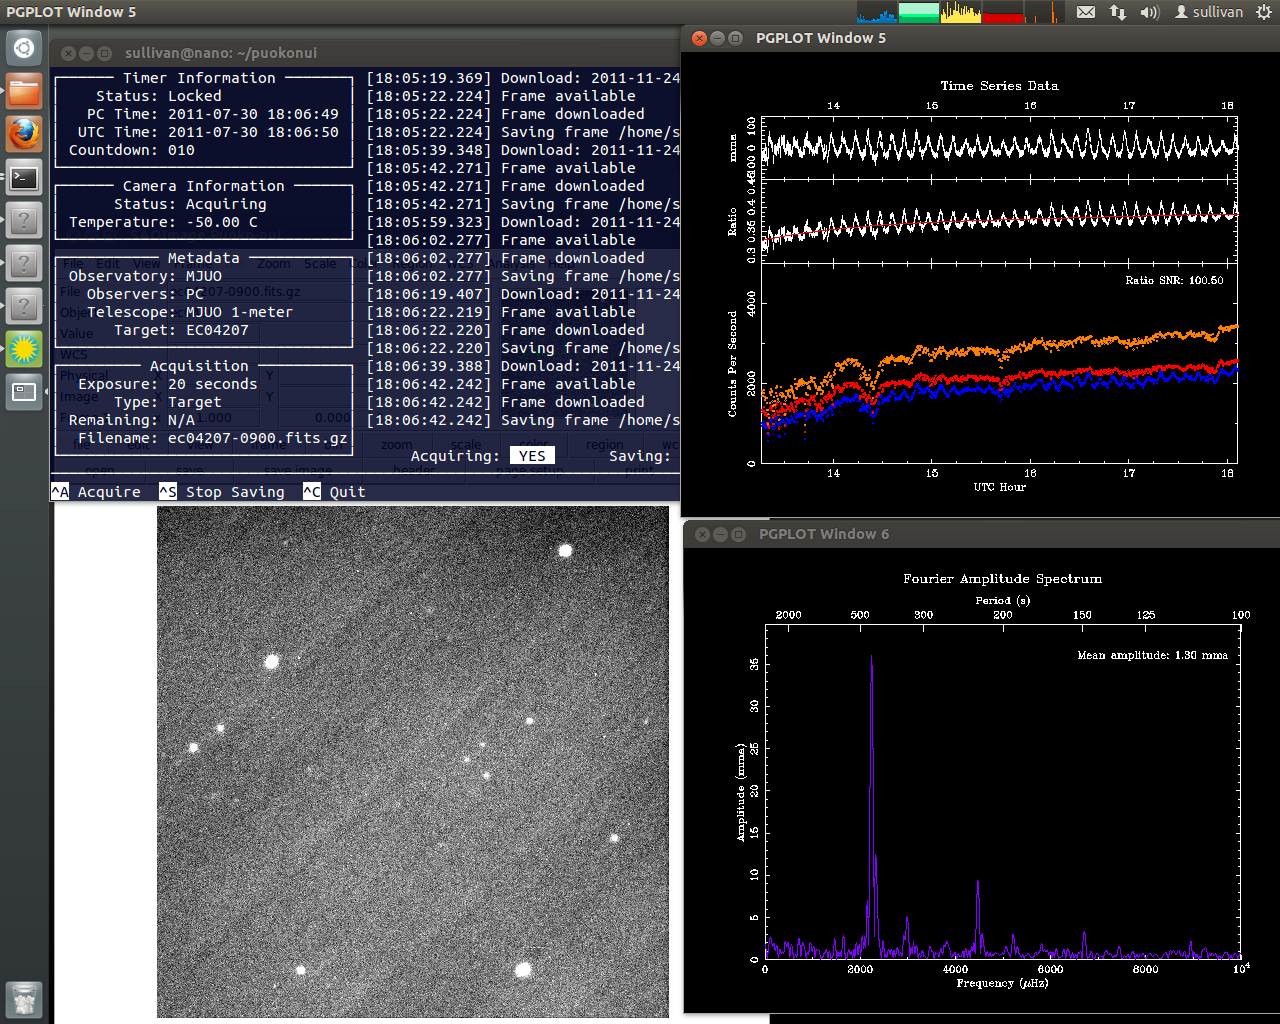
\includegraphics[width=\textwidth]{figures/screenshot}\\
						\small The instrument control software and online reduction as visible during an acquisition run
					\end{beamercolorbox}
					\vskip 4.5ex
					\begin{block}{\large Acknowledgements}
						\justifying
						%!TEX root = /Users/paul/phd/talks/WD12poster/puokonui-poster.tex
\vspace{-1.75cm}
\begin{itemize}[itemsep=20pt]
\item[] We thank the University of Canterbury in New Zealand for providing
access to the Mt John facilities and the NZ Marsden Fund for their generous
financial support.
\end{itemize}
\vspace{-1.75cm}
					\end{block}
				\end{column}
			\end{columns}
		\end{adjustbox}
		\vskip -3ex
	\end{frame}
\end{document}